    \subsection{Support Vector Machines}
        Method that originates from linear programming:
        \begin{itemize}
            \item Objective function 
            \item Constraints 
        \end{itemize}
        SVMs aim at maximizing the margin to pull both classes as far apart as possible.\\
        We call \textbf{support vectors} the training points that lie on the separating hyperplanes.\\
        The optimization problem has a quadratic cost function, no local minima and only one global minimum.\\
        In the real world it exists the non-linear separable case, add an error term to consider how much are we misclassifying, use kernel function to change feature space.
        \subsubsection{Interpretability and Variable Selection}
            They are black box methods, complex in settings where interpretability is important.\\
            Variable selection can be performed using backward variable selection (this reduces the variables but not provide any additional insight into the workings of the SVM).
        \subsubsection{Rule Extraction}
            \begin{itemize}
                \item \textbf{Decompositional:} represent SVM as a neural network
                \item \textbf{Pedagogical:} 
                \begin{itemize}
                    \item Use SVM first to construct a dataset with SVM predictions for each one of the observations
                    \item Give the dataset to a decision tree algorithm to build a decision tree
                \end{itemize}
                \item \textbf{Two stage models:} A simple model is estimated first, followed by a SVM to correct the errors of the latter
            \end{itemize}
    \subsection{Ensemble Methods}
        The idea is to provide an explanation of the target label by putting toghether different models combining their results, based on the assumption that multiple diverse models capture different trends of the dataset.\\
        To be successful, ensemble must be done with models sensitive to changes.
        \begin{itemize}
            \item \textbf{Bagging}
            \item \textbf{Boosting}
            \item \textbf{Random Forests}
        \end{itemize}
        \subsubsection{Bagging}
            \begin{itemize}
                \item Start by taking B bootstraps from the underlying sample. A bootstrap is a sample with replacement.
                \item Build a model for every bootstrap
                \item Use majority voting for classification, average for regression
            \end{itemize}
            The key element for bagging is the instability of the analytical technique. For models that are robust with respect to the underlying dataset, bagging will not give much added value.
        \subsubsection{Boosting}
            Estimate multiple models using a weighted data sample \textit{(uniform at the beginning)}.\\
            Iteratively re-weight data according to classification error.\\
            The idea is that difficult observations should get more attention. The final ensemble is a weighted combination of all the individual models.
            \begin{itemize}
                \item Key Advantage: easy to implement
                \item Potential Drawback: risk to overfitting to the hard \textit{(potentially noisy)} examples in the data, which will get higher weights as the algorithm proceeds. Relevant in fraud detection setting because the target labels are tipically quite noisy.
            \end{itemize}
        \subsubsection{Random Forests}
            Creates a forest of decision trees:
            \begin{itemize}
                \item Given a dataset with n observations and N inputs 
                \item m = constant chosen on beforehand 
                \item For t = 1,\dots,T:
                \begin{itemize}
                    \item take a bootstrap sample with n observations 
                    \item build a decision tree whereby for each node of the tree, randomly choose m variables on which to base the splitting decision
                    \item Split on the best of this subset 
                    \item Fully grow each tree without pruning
                \end{itemize}
            \end{itemize}
            Create as much diversity in the classifiers, the higher the diversity, the higher the performances.
        \subsubsection{Evaluating Random Forests}
            Random forests can achieve excellent predictive performances.\\
            Their main disadvantage is that they are black-box models because they're based on random decision trees.
\section{Evaluating a Fraud Detection Model}
    When evaluating predictive models, two key decisions need to be made:
    \begin{itemize}
        \item \textbf{On the dataset split up}
        \item \textbf{On the performance metrics}
    \end{itemize}
    \subsection{Splitting up the dataset}
        \subsubsection{Large dataset}
            The decision on how to split up the dataset for performance measurements depends on its size.\\
            Split large datasets into:
            \begin{itemize}
                \item (70\%) Training dataset 
                \item (30\%) Test dataset
            \end{itemize}
            There must be \textbf{strict separation} between training and test sample.\\
            In the case of decision trees or neural networks separate the training dataset in 40\% training, 30\% validation.\\
            Stratified split-up ensures that fraudsters/non-fraudsters are equally distributed amongst the various samples.
        \subsubsection{Small dataset}
            With small datasets special schemes need to be adopted
            \begin{itemize}
                \item \textbf{Cross-validation:} split data in K folds, train models with K-1 folds and test on the remaining one. It will result in K performance estimates that then are averaged.
                \item \textbf{Leave-one-out cross-validation:} every observation is left out in turn and a model is estimated on the remaining K-1 observations, this gives K analytical models in total.
            \end{itemize}
            Cross-validation gives multipe models, how should the final model be?
            \begin{itemize}
                \item All models collaborate in an ensamble 
                \item Pick one LOO model at random, they will be quite similar anyway
                \item Build one final model on all observations but report the performance coming out of the cross-validation
            \end{itemize}
    \subsection{Performance Metrics}
        \begin{itemize}
            \item \textbf{Classification Accuracy:} percentage of correctly classified observations: $$\frac{TP+TN}{TP+FP+FN+TN}$$
            \item \textbf{Classification Error:} $$\frac{FP+FN}{TP+FP+FN+TN}$$
            \item \textbf{Sensitivity, Recall or Hit Rate:} how many of the fraudsters are correctly labeled as fraudster: $$\frac{TP}{TP+FN}$$
            \item \textbf{Specificity:} how many of the non-fraudsters are correctly labeled as non fraudsters $$\frac{TN}{FP+TN}$$
            \item \textbf{Precision:} how many of the predicted fraudsters are actually fraudsters $$\frac{TP}{TP+FP}$$
        \end{itemize}
        Usually accuracy is not a good measure in fraud detection domain because frauds are rare, disperse in a huge amount of data.\\
        Frauds represent 0.1 percent of data, if you say that everything is legitimate you will still get an accuracy of 99,9.\\
        The good measures are F1 measure: armonic mean of precision and recall, Matthew Correlation Coefficient or other graphical measures and precision/recall.
        \subsubsection{Receiver Operating Characteristic (ROC) Curve}
            It plots the sensitivity vs 1-specificity:
            \begin{figure}[ht!]
                \centering
                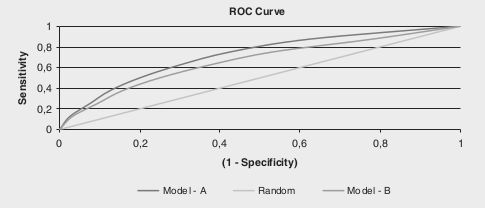
\includegraphics[width=0.6\linewidth]{lecture_16/roc.png}
            \end{figure}
            a good model will be near to the extreme left point of the graph.\\
            A problem arises if curves intersect, \textbf{AUC (Area under the ROC curve)} provides a simple figure-of-merit for the performance:\\
            the higher the AUC, the better the performance. It interprets the probability that a randomly chosen fraudster gets a higher score than a randomly chosen nonfraudster.\\
            A good classifier should have a ROC above the diagonal, and AUC bigger than 50\%.
    \subsection{Developing predictive models for skewed datasets}
        Fraud detection datasets often have a very skew target class, frauds are $$\leq 1\%$$. This creates problems for the analytical techniques.\\
        It is recommended to increase the number of fraudulent observations or their weight, such that the analytical techniques can pay better attention to them.\\
        Increase the number of frauds by:
        \begin{itemize}
            \item Increasing the time horizon for prediction: instead of six-month, 12-month.
            \item Sample every fraud twice or more 
            \item Undersample the majority case
        \end{itemize}
        \subsubsection{Oversampling}
            Replicate frauds two or more times to make the distribution less skew
        \subsubsection{Undersampling}
            Remove nonfrauds two or more times to make the distribution less skew, remove low value transactions or inactive accounts.
        \subsubsection{Under and Over sampling}
            They can be combined, they should be performed only on training data and not on test data to give an unbiased view on model performance.
        \subsubsection{SMOTE: Synthetic Minority Oversampling Technique}
            Works by creating synthetic observations based on the existing minority observations.\\
            Synthetically generate new samples from the ones available, identify the k nearest neighbors from the sample to replicate and synthetically generate the new one averaging the neighbors.
        \subsubsection{Cost-Sensitive Learning}
            Besides interpretability, efficiency is the main problem:\\
            output is going to be investigated. We can estimate the cost associated to the misclassification 
            \begin{figure}[ht!]
                \centering
                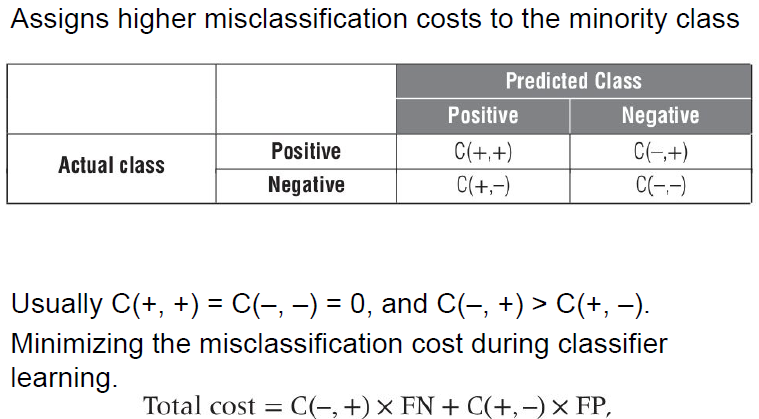
\includegraphics[width=0.6\linewidth]{lecture_16/last.png}
            \end{figure}